	\chapter{Detalles de implementaci\'on}

\section{Introducci\'on}

En el siguiente cap\'itulo describiremos los detalles del trabajo realizado, desde la estructuraci\'on de las fuentes de datos utilizados, hasta la implementaci\'on de los algoritmos de b\'usqueda.Dado que el objetivo principal de \'este trabajo es determinar (a trav\'es de la aplicaci\'on a un caso de uso real) que estrategia de selecci\'on de pivotes es la mejor, nos restringimos a implementar el m\'etodo b\'asico de b\'usqueda que puede utilizarse para realizar b\'usquedas desde cualquier tipo de sistema: sitio web, aplicaci\'on de tel\'efono celular, etc.\\

Para el desarrollo del software seleccionamos el framework Grails (versi\'on 1.3.7), que contiene el lenguaje Groovy para la codificaci\'on y Java para la ejecuci\'on.\\

Todas las estructuras de datos fueron manejadas en memoria principal, tanto para la creaci\'on de \'indices como para las b\'usquedas.


\section{Procesamiento inicial de los datos de entrada}

Cuando hablamos de datos de entrada, nos referimos a los productos ofrecidos en el sitio MercadoLibre (a los que tambi\'en llamaremos items). Estos productos est\'an clasificados dentro de un \'arbol de categor\'ias, donde cada categor\'ia re\'une productos relacionados. Remitiendonos a los n\'umeros, obtuvimos alrededor de 2 millones de productos, distribuidos en 12.000 categor\'ias (hojas).\\

La informaci\'on relevante a \'este trabajo obtenida de los productos fue la siguiente: categor\'ia, identificador del producto, t\'itulo, descripci\'on principal y descripci\'on secundaria.\\

Para optimizar el desarrollo de creaci\'on de \'indices, los datos de entrada tuvieron que ser pre-procesados para crear los archivos necesarios para el correcto funcionamiento de dicho proceso. De este pre-procesamiento obtuvimos:\\

\begin{enumerate}[(1)]
\item  Archivo de productos: texto plano conteniendo toda la informaci\'on pertinente de los productos, separada por comas.
\item  Archivo de categor\'ias: texto plano conteniendo el nombre de la categor\'ia.
\item  Archivo de productos divididos por categor\'ia: archivo de datos serializados, conteniendo un mapa cuyas claves son las categor\'ias y cuyo valor es la lista de productos correspondiente, conteniendo informaci\'on m\'inima para la selecci\'on de pivotes: identificador del producto y codificaci\'on del t\'itulo (la codificaci\'on consiste en eliminar caracteres especiales, reemplazar vocales acentuadas por no acentuadas, suprimir espacios superfluos y pasar a may\'usculas el t\'itulo completo).
\end{enumerate}

\section{Estructuras de datos}

Para el almacenamiento de las categor\'ias se implement\'o un rebalse abierto lineal con un factor de carga de 0.4.
Cada elemento del rebalse se compone de una estructura que contiene el nombre de la categor\'ia y una lista de firmas. Cada firma representa la distancia de edici\'on de cada t\'itulo del \'item a cada t\'itulo del elemento pivote, e incluye el identificador de \'item en cuesti\'on.\\

Por otro lado, para el almacenamiento de los datos completos del producto se utiliz\'o un mapa cuya clave es el identificador y el valor asociado es una estructura que contiene la totalidad de los datos del producto.\\

Como \'ultima estructura de datos auxiliar, se eligi\'o un mapa cuya clave es la categor\'ia y el valor asociado es la lista de pivotes correspondiente, conteniendo solo el identificador del producto y la codificaci\'on del t\'itulo.\\

\begin{figure}[H]
\centering
\subfigure[\scriptsize Rebalse de categor\'ias]{
\includegraphics[width=71.5mm]{imagenes/estructuras/categs-hash.png}}
\subfigure[\scriptsize Mapa de productos]{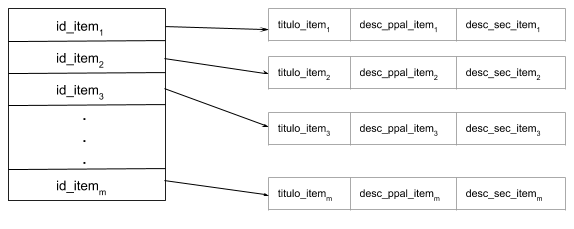
\includegraphics[width=71.5mm]{imagenes/estructuras/map-items.png}}
\subfigure[\scriptsize Mapa de pivotes por categor\'ias]{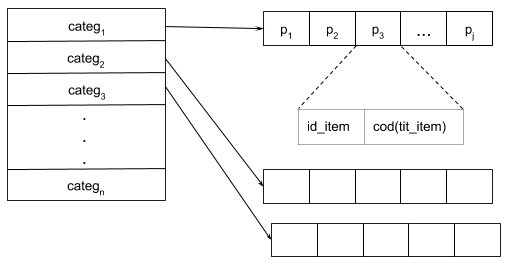
\includegraphics[width=71.5mm]{imagenes/estructuras/categs-pivots.png}}
		\caption{\small Estructuras de datos utilizadas}
		\label{fig:estructuras}
\end{figure}

\section{Software desarrollado}

El desarrollo realizado consta de dos partes complementarias: la funcionalidad de creaci\'on de \'indices y la funcionalidad de b\'usqueda propiamente dicha, que utiliza los \'indices creados por la primera funcionalidad.\\



\subsection{Creaci\'on de \'indices para las b\'usquedas}

La funcionalidad de creaci\'on de \'indices se desarroll\'o en forma gen\'erica, preparada para recibir los siguientes par\'ametros: tipo de pivotes (random o incremental), cantidad de pivotes y conjunto de pivotes (mismo conjunto para todas las categor\'ias o diferentes conjuntos para cada categor\'ia)\\

La l\'ogica b\'asica del algoritmo de creaci\'on de \'indices carga los archivos descritos en la secci\'on  \textbf{Procesamiento inicial de los datos de entrada} en las estructuras de datos correspondientes, y procede a generar las firmas de los items, utilizando en primera instancia la estrategia de selecci\'on de pivotes en conjunci\'on con el resto de los par\'ametros (cantidad y conjunto de pivotes). Luego de completar la estructura con las firmas de los items, almacena cada estructura en un archivo de datos serializados; para que puedan ser utilizados en futuras b\'usquedas.\\

De \'esta manera, el algoritmo de creaci\'on de indices particiona el universo de datos U (los productos) a trav\'es de las categor\'ias hojas, resultando en multiples U-i listas que potencialmente contienen elementos relevantes para una consulta.\\






\textbf{////////////////AGREGAR PSEUDOCODIGO///////////}








\subsection{Busqueda por similitud}

Se implementaron dos funcionalidades de b\'usqueda: b\'usqueda por rango, que recibe por par\'ametro el radio de b\'usqueda, la categor\'ia del producto y el t\'itulo de un producto existente; y b\'usqueda de los k-vecinos, que recibe por par\'ametro la cantidad de elementos a retornar (k), la categor\'ia del producto y el t\'itulo de un producto existente.\\

La b\'usqueda por rango calcula la distancia del t\'itulo del producto dado por par\'ametro a cada uno de los pivotes, y luego compara esa firma contra las firmas de los productos de la categor\'ia seleccionada. Este paso devuelve los productos candidatos a formar parte de la respuesta final, los cuales son utilizados para calcular la distancia real de edici\'on contra el producto buscado, descartando aquellos que est\'en fuera del rango especificado.\\

La b\'usqueda de los k-vecinos utiliza una variaci\'on de la b\'usqueda por rango, comenzando con un rango de 5 e incrementando ese valor hasta llegar a la cantidad deseada de resultados.\\

Como funcionalidad auxiliar, se implement\'o un proceso de carga que puede ser utilizado al iniciar el programa, para cargar los archivos de \'indices previamente generados.\\





\textbf{////////////////AGREGAR PSEUDOCODIGO///////////}






\section{Re-particionado del universo}

Luego de planificar y diseñar e implementar todas las estructuras de datos, realizamos pruebas manuales para asegurarnos del correcto funcionamiento del software completo.\\

Ante \'estas pruebas, detectamos que el particionado no era sem\'anticamente correcto, ya que al elegir la categor\'ia hoja del \'arbol, estabamos restringiendo demasiado el universo de b\'usqueda. Representando la situaci\'on con un ejemplo, supongamos que deseamos recomendar productos similares al producto \textit{“Samsung Galaxy A30 32 GB Blanco 3 GB RAM”}, la categor\'ia hoja de dicho producto es \textit{“A30”}, dentro del \'arbol: \textit{“Celulares y Tel\'efonos > Celulares y Smartphones > Samsung > A30”}, si solo tenemos en cuenta los productos que pertenecen a la categor\'ia \textit{“A30”}, es probable que no encontremos, por ejemplo, celulares blancos de 32 GB de la marca Motorola.
Por \'este motivo, definimos volver a particionar el universo de productos, \'esta vez utilizando la categor\'ia inicial del \'arbol (Celulares y Tel\'efonos en el ejemplo anterior).\\

Con \'esta nueva estrategia, obtuvimos 30 particiones distintas de nuestro universo, para las cuales realizamos los experimentos descritos en el pr\'oximo cap\'itulo.
